% Metódy inžinierskej práce

\documentclass[10pt,twocolumn,twoside,english,a4paper]{article}

\usepackage[english]{babel}
%\usepackage[T1]{fontenc}
\usepackage[IL2]{fontenc} % lepšia sadzba písmena Ľ než v T1
\usepackage[utf8]{inputenc}
\usepackage{graphicx}
\usepackage{subcaption}
\usepackage{url} % príkaz \url na formátovanie URL
\usepackage{hyperref} % odkazy v texte budú aktívne (pri niektorých triedach dokumentov spôsobuje posun textu)

\usepackage{cite}
%\usepackage{times}

\pagestyle{headings}

\title{Recommendation systems for personalized advertising in digital marketing} % meno a priezvisko vyučujúceho na cvičeniach


\author{Vsevolod Salik\\[2pt]
	{\small Slovak University of Technology in Bratislava }\\
	{\small Faculty of Informatics and Information Technologies }\\
	{\small \texttt{xsalik@stuba.sk}}
	}

\date{\small 26. september 2024} % upravte



\begin{document}


\maketitle
%\thanks{Semestral project in the subject Methods of engineering work, academic year 2024/25, supervised by Pavol Batalik}
%insert thanks part in the title after i figure out how it works


\begin{abstract}
\ldots
\end{abstract}



\section{Introduction}


\section{ImagesTest}
\graphicspath{ {./images/PNG} }
Inserted image using basic includegraphics


\includegraphics[width=0.5\textwidth]{STU-FIIT-ancnh.png}

I needed to use [h] for my second image so it doesnt go to the end of the file, that why there is weird identation

\begin{figure}[h]
	
\includegraphics[width=0.5\textwidth]{STU-FIIT-anfnh.png}
	\caption{STU FIIT Logo blue version}
	\label{logo_2}
\end{figure}

\hfil
\includegraphics[width=0.3\textwidth]{STU-FIIT-ancnv.png}\hfil
\includegraphics[width=0.3\textwidth]{STU-FIIT-ancv.png}

\section{Practice 4}

\begin{figure}[h]
	\caption{All variations of FIIT LOGO}
	\label{fig:logos}
	\begin{subfigure}[b]{0.3\textwidth}
		
\includegraphics[scale=0.3]{STU-FIIT-nfv.png}
		\caption{Blue version}
	\end{subfigure}
	\begin{subfigure}[b]{0.3\textwidth}
		
\includegraphics[scale=0.3]{STU-FIIT-zcv.png}
		\caption{White version}
	\end{subfigure}
	\begin{subfigure}[b]{0.3\textwidth}
		\centering
		
\includegraphics[scale=0.3]{STU-FIIT-zcvn.png}
		\caption{Black version}
	\end{subfigure}
\end{figure}

\begin{figure*}[h]
	\caption{UMLet diagrams}
	\label{fig:umletdiag}
	\begin{subfigure}[b]{0.5\textwidth}
		\centering
		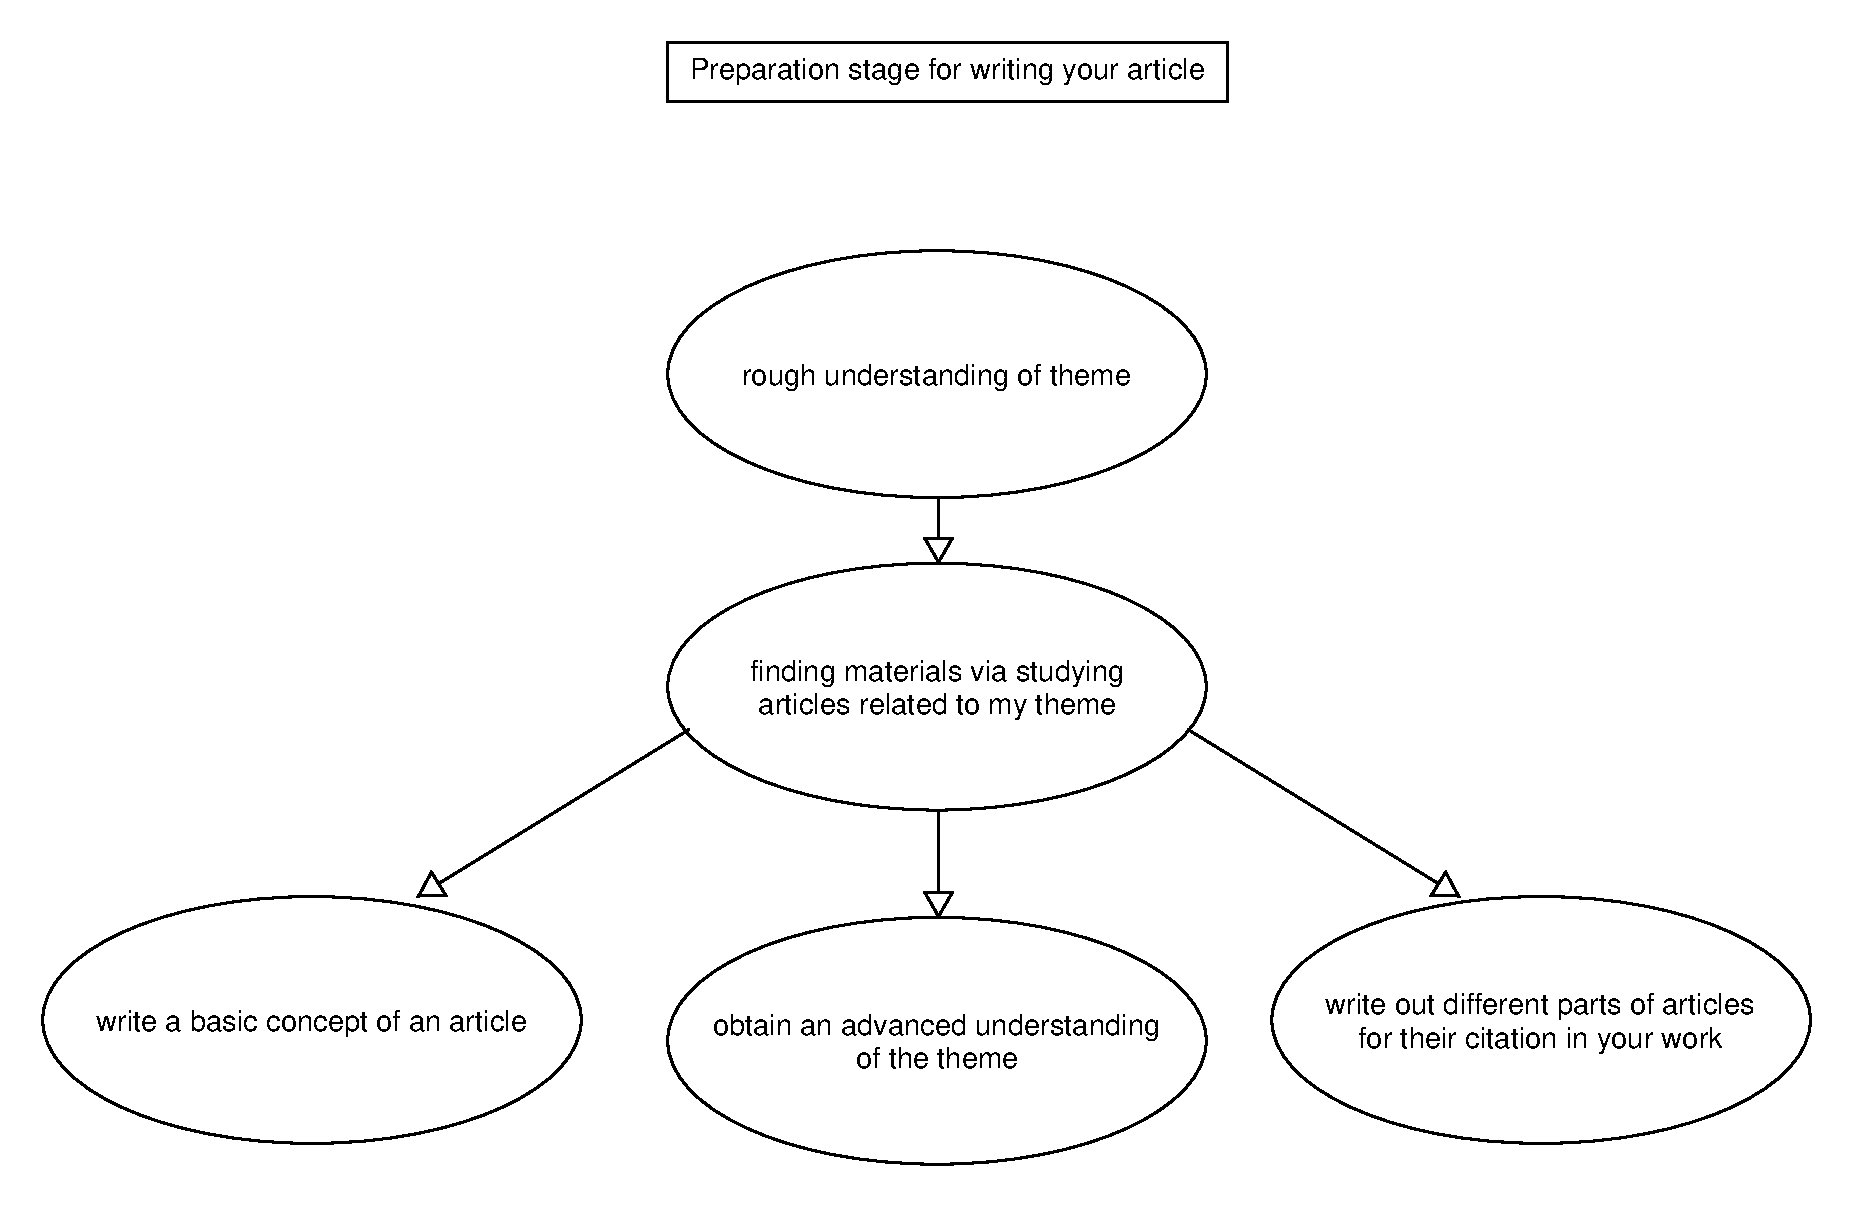
\includegraphics[width=1\textwidth]{diagram_1.pdf}
		\caption{diagram n.1}
	\end{subfigure}
	\begin{subfigure}[b]{0.5\textwidth}
		\centering
		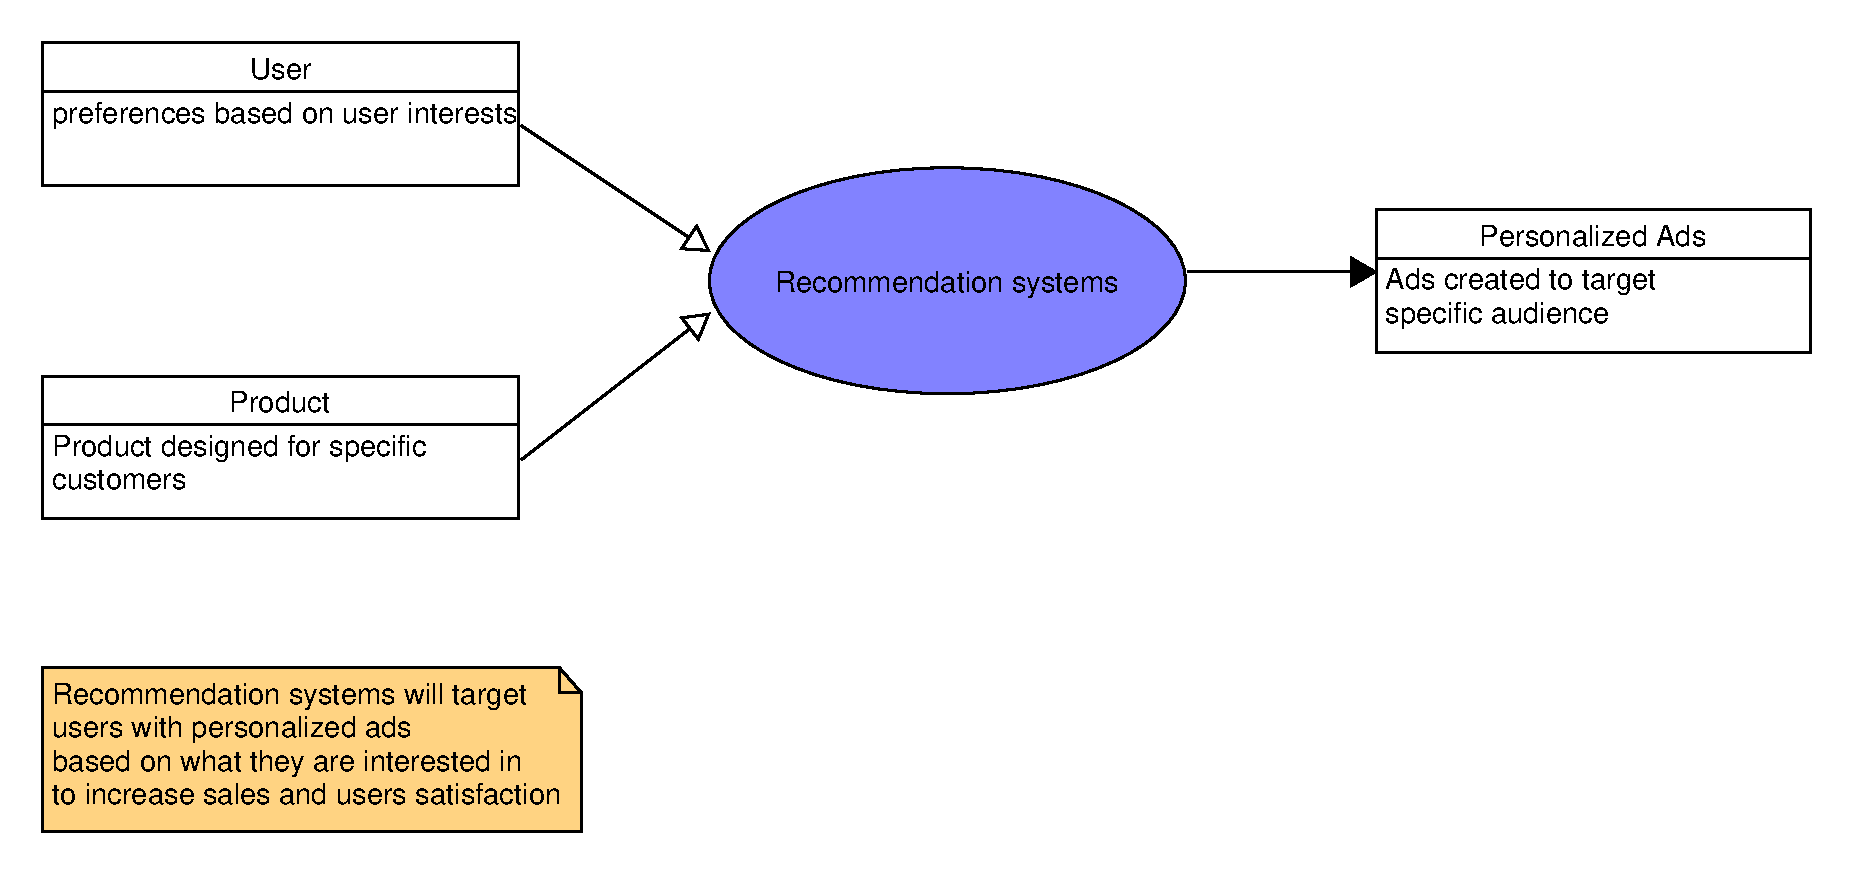
\includegraphics[width=1\textwidth]{diagram_2.pdf}
		\caption{diagram n.2}
	\end{subfigure}
\end{figure*}

%\acknowledgement{Ak niekomu chcete poďakovať\ldots}


% týmto sa generuje zoznam literatúry z obsahu súboru literatura.bib podľa toho, na čo sa v článku odkazujete
% \bibliography{literature}
% \bibliographystyle{plain} % prípadne alpha, abbrv alebo hociktorý iný
\end{document}
